% !TeX root = ../thuthesis-example.tex

\chapter{车辆信誉评估算法的设计}

在已有工作中,多数车辆信誉评估的相关算法都基于车辆单独的驾驶行为,或者只针对在行驶过程中车辆某种特定的行为,车载网中大量的信息交换没有得到充分利用。本章提出了一套基于车辆交互结果的信誉评估算法,主要由交互活跃度、位置验证结果、消息传播结果三部分构成,同时通过对具体场景的讨论分析算法的科学性与可靠性。

\section{基本设计思路}
\subsection{信誉值影响因素}

车辆在行驶过程中携带了大量信息,如何筛选这些信息、保留对于车辆信誉最具有代表性的关键因素是设计该算法的第一个问题。考虑到车辆信誉值本质上是其他车辆用于决定是否信任该车辆的判断指标,车辆在自组网中参与的信息交互结果应当是信誉评估的主要影响因子。而一辆车自身的行驶状态,譬如行驶速度、运动轨迹、驾驶员操作等信息,尽管可以对信誉判断起到辅助作用,但是不属于展现该车对邻近车辆是否可信的主要参考指标,通常也无法直接地反映其信誉;因此,为了保证算法的简洁性,这类因素不属于笔者进行算法设计时的考量目标。

本文提出的车辆信誉算法主要受到以下几个因素的影响:

\begin{enumerate}
    \item 用户活跃度。车辆上传有效数据、更新状态的频率越高,其对应的信誉增益就更加明显,这代表它在车载网中积极地进行信息交互,并且共享的信息频繁地得到了其他车辆的确认。如果车辆很少在网络中与其他车辆进行任何互动,那么极其稀疏的数据提交对其信誉增长的帮助将是非常有限的:一方面是由于车辆的信誉同样具有时效性,在计算时需要保证信誉值能准确地体现车辆当前的可信程度,用户长时间的沉寂会使其历史信誉不再具有足够的效力;另一方面可以防止恶意车辆用户和少量的同谋伪造有效信息,仅通过少量的数据提交就能获得很好的信誉评价。
    \item 车辆交互的结果。这是本文算法进行信誉评估的主要计算依据,因为车辆之间进行信息交互的结果、邻近车辆对于信息的评价是直接体现车辆可信度的指标。其中,车辆的交互方式主要包括:
    \begin{enumerate}
        \item 位置验证。车载网在应用中包含众多基于位置的服务,因此位置验证是车辆行驶过程中进行得较为频繁的一项例行交互行为。车辆通过短距离通信向邻近车辆发送请求,表示自己希望得到位置验证,然后邻近车辆根据自身的定位信息和请求者提供的地理位置,返回经过自己确认的验证结果,可以视为一次成功的位置验证。成功的位置验证可以确认车辆提供的地理位置信息的准确性,以及在对应的信息交换过程中的诚实行为,从而得到信誉值的提升;相反,位置验证失败可能意味着车辆自身定位不够准确、车辆故意捏造虚假的位置信息等状况,但无论如何,验证失败都代表车辆提供的信息对于网络中的其他用户来说是不够可信的,因此其信誉值会相应减少。
        \item 消息传播。车辆之间传播的消息,譬如路况提示、事故告警等,其发生频率低于位置验证,但同样是衡量车辆可信度的重要指标。车辆的信誉由其发送消息的质量(准确性、及时性)体现,每条消息的质量通过其他收到消息的车辆对其给出的评价来确定,而周围车辆给出的评价是否客观准确,则和它与消息发送者之间的距离相关。
    \end{enumerate}
    \item 监督与举报。上述车辆交互通常限于两辆车之间,但是为了防止恶意信息的伪造和传播,车辆信誉评估的系统同样鼓励第三方对交互内容的监督和举报。不论是位置验证还是消息传播,相关数据都将在车载网内部进行传播,收到信息的第三方车辆可以对其内容进行检查,并举报虚假信息的存在。由于这一行为需要用户额外的计算开销,因此举报成功可以获得相应的信誉值奖励,同时被举报的恶意用户将受到严厉的惩罚。
\end{enumerate}

\subsection{交互模型与算法流程}

该算法对应的车辆交互模型如图~\ref{fig:model}所示。该模型中,信誉计算的参与方包括三种对象:目标车辆,信誉值所评估的直接对象;邻近车辆,与目标车辆进行过交互、并提交结果的车辆;路侧单元(RSU),收集车辆数据、完成信誉计算的对象。目标车辆可向邻近车辆发送位置验证请求,或进行消息的传播,对于两种交互方式,邻近车辆分别给出位置验证的结果或者对于消息的评价。算法中包含基于两种交互模式的信誉计算方案,对交互结果在RSU中分别进行相应的处理,最后将计算得到新的信誉值传输给目标车辆。

在实际应用中,RSU使用区块链结构进行信誉维护,使得信誉评估的过程得到安全性的保障。在目标车辆完成一次与邻近车辆的交互后(如进行一次位置验证,或发送一条消息),交互结果被上传到RSU,并根据本章提出的算法进行信誉偏移值的计算,并更新目标车辆的信誉值。

图~\ref{fig:algo}具体展现了RSU中两个计算模块对应的算法流程。其中,位置验证模块根据当次及历史的验证结果完成信誉偏移值的计算,而消息评价模块首先根据每个邻近车辆分别给出的消息评价以及它们与目标车辆之间的距离,计算出该消息的总评价,然后再计算信誉偏移值。时间衰减系数由用户提交数据的间隔计算得到,在两个模块中分别与对应的信誉偏移值进行叠加,得到最终的信誉计算结果。下一节将对具体的计算公式进行介绍。

\begin{figure}
  \centering
  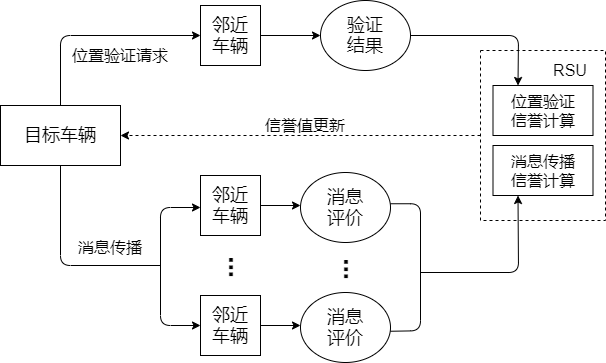
\includegraphics[width=0.8\linewidth]{figures/model.png}
  \caption{信誉评估算法交互模型示意图}
  \label{fig:model}
\end{figure}

\begin{figure}
  \centering
  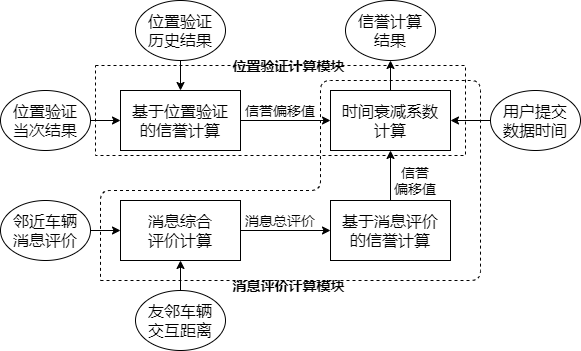
\includegraphics[width=0.8\linewidth]{figures/algo.png}
  \caption{信誉评估算法流程图}
  \label{fig:algo}
\end{figure}

\section{信誉计算方式}

本节将介绍车辆信誉算法涉及到的具体公式。将目标车辆的信誉值记为$T$,$T$是在$[0,100]$范围内的整数。在目标车辆作为新用户加入到车载网中时,它被赋予初始信誉值$T_0$。每次进行位置验证或消息传播后,车辆间交互的结果将被用于计算目标车辆新的信誉值$T'$。下面介绍信誉值更新的具体算法。

\subsection{时间衰减系数}
目标车辆基于一次交互更新的信誉值为:

\begin{equation}
    T'=T+\Delta T*D(t)
    \label{eq:credit}
\end{equation}

其中$T$为本次信誉计算前车辆的原始信誉值,$\Delta T$为根据本次交互结果计算得到的信誉偏移值,$D(t)$表示基于数据提交时间间隔得到的时间衰减系数,其计算方法如下:

\begin{equation}
    D(t)=\frac{1}{\delta*(t-t_l)}
    \label{eq:timedecay}
\end{equation}

其中$\delta$为参数,$t$表示本次提交数据的时间,$t_l$表示上一次提交数据的时间。通过公式\eqref{eq:timedecay}引入时间衰减系数,目的在于以数据提交时间间隔对用户活跃度进行量化。在公式\eqref{eq:credit}中将信誉偏移值与时间衰减系数进行叠加,使得活跃度这一指标在信誉调整的幅度上能够得到明确的体现,而同时避免了交互结果对信誉的影响被完全覆盖:成功的交互必然能导致信誉提升,失败的交互必然能导致信誉下降,但是交互的频率作用于信誉的增减幅度,长时间不提交数据会导致一次交互结果对信誉值的总影响减弱。

\subsection{基于位置验证的信誉计算}
在目标车辆进行一次位置验证之后,其信誉偏移值的计算方式如下:

\begin{equation}
    \Delta T=\left\{\begin{aligned}
    &max(\theta_{s}*(sRate+1)+\theta_{f}*fRate,0), & \mbox{本次验证成功}\\
    &min(\theta_{s}*sRate+\theta_{f}*(fRate+1),0), & \mbox{本次验证失败}\\
    \end{aligned} \right.
    \label{eq:locproof}
\end{equation}

其中$sRate$、$fRate$分别表示目标车辆在近期一段行驶历史中位置验证的成功率和失败率。该公式保证了本次验证结果对信誉偏移方向的决定性影响:本次验证成功必然使信誉提升,本次验证失败必然使信誉下降。除了对当次位置验证结果进行考量之外,\eqref{eq:locproof}还引入了历史记录中的验证结果,在保证本次验证占有最大权重的同时对信誉偏移的计算结果进行平滑处理。

\subsection{基于消息传播的信誉计算}
在目标车辆i向周围车辆发送一条消息m之后,收到这条消息的邻近车辆j将根据消息内容的准确性对其进行打分,分数$R_j^m$为$[1,10]$之间的整数。在汇总了所有周围车辆对消息m的打分之后,可计算其总评价:
\begin{equation}
    Cred_m=\frac{\sum_jw_{ij}*R_j^m}{\sum_jw_{ij}}
    \label{eq:messagecred}
\end{equation}

其中权重$w_{ij}$由车辆$i$、$j$的距离$dis(i,j)$决定:
\begin{equation}
    w_{ij}=e^{-\gamma* dis(i,j)}
    \label{eq:disweight}
\end{equation}

在公式\eqref{eq:messagecred}中,对邻近车辆的打分进行加权的意义在于,邻近车辆对消息内容的评价应当基于自己对实际情况的观察,因此其评价与自身和消息相关事件之间的距离也有一定关系。考虑到这条消息描述的是目标车辆所处位置的事件,故可用目标车辆和邻近车辆之间的距离表示消息描述事件和消息评价者之间的距离。从公式\eqref{eq:disweight}中可以看出,两辆车距离越近,对应的消息打分所占权重越高,代表该邻近车辆对事件的观察、对消息的评价更具有说服力。

在计算得到消息m的总评价后,可根据$Cred_m$判定消息是否可信,从而计算相应的信誉偏移值:

\begin{equation}
    \Delta T=\left\{\begin{aligned}
    &Reward=\alpha*D*\frac{1}{e^L}, &{Cred_m\geq C_0,\mbox{消息可信}}\\
    &Punishment=(-1)*\beta*D*\frac{1}{e^L}, & {Cred_m<C_0,\mbox{消息不可信}}\\
    \end{aligned} \right.
    \label{eq:message}
\end{equation}

其中$C_0$为参数,$D$表示车辆密度,$L$表示消息的紧急级别($L=1$:事故警告;$L=2$:路况提示)。可以看到,车辆密度越大、消息内容越紧急,计算得到的信誉偏移幅度就越大,因为有更多的车辆受到了这条消息的影响。

\section{科学性分析}

当车辆在道路上正常行驶,并能够持续、稳定地与周围车辆完成交互时,该算法显然能保证目标车辆信誉值的稳步上升;然而实际应用中,可能会遇到各种特殊情况,不论是否是人为制造,都会导致车辆交互失败并使其信誉值下降。本节将针对一些可能出现的意外情况进行具体讨论,分析上文提出的算法是否能在这些情况下合理、公正地体现车辆信誉的变化。

\begin{enumerate}
    \item 客观原因导致交互失败。目标车辆可能由于自身设备出现故障等原因,导致无法获取准确的地理位置信息,或者中断与其他车辆的通讯,进而导致信誉值的下降。这种情况的出现,并不违背本文算法设计的前提:车辆信誉值是为其他车辆提供的、用于判断该车辆提供信息是否可信的评价指标,即使是由于客观原因导致的交互失败,也意味着目标车辆当前的状况并不适合与其他车辆共享信息。对于个别偶然的失败情况来说,本文算法引入了历史记录进行偏移值的平滑,这使得拥有良好交互记录的车辆不会大幅损失信誉值;如果在一段时间内存在持续的失败交互,车辆的信誉值将降低至不可信水平,但是如果影响车辆的客观因素消失,其信誉值还能够通过之后的正常活动重新回升。
    \item 恶意诋毁。道路上可能存在一些恶意的车辆,在作为邻近车辆参与交互时故意给予负面的反馈,譬如声称其他车辆位置验证请求中的地理信息不合法,或者故意给其他车辆发出的消息打出低分。本文算法没有为了避免这种情况而进行专门的设计,但是可以看到当这种恶意车辆在整体交通中仅占少数部分时,它们的诋毁行为不会对诚实车辆的信誉产生明显的影响。对于位置验证,考虑到历史验证成功率对整体结果的平滑,个别的验证失败结果对车辆可信度影响不大。对于消息传播,消息总评价由多车打分的加权平均得到,并且最终只通过消息是否可信来判定信誉值增减,而不考虑可信范围内具体的分数高低。因此,少数的恶意负面评价通常也很难影响最后的整体结果。
    \item 多人合谋。车载网系统中还可能面临的一种安全威胁,是多台恶意车辆之间的合谋,例如一台恶意车辆可以发送包含虚假位置信息的位置验证请求,而其合谋者为其提供捏造的确认信息,两者通过这种形式完成了一次成功的位置验证并获得了信誉值的提升,尽管验证的信息实际上并不合法。对于本文提出的算法来说,这种形式的攻击仅当与之合谋的车辆足够多时才能够收获明显的效果。这是因为区块链上维护了一段时间内的车辆交互结果记录,而同一对车辆在这段时间内不能反复地进行同样的交互。如果其他车辆能够正常地识别恶意车辆信息的异常,那么这种合谋行为也难以有效地提升其信誉值,除非周围的车辆都是与之串通的共犯;但是在实际情况中,这样做的伪造成本会变得极其高昂,再考虑到车辆的流动,其可行性也是较低的。
\end{enumerate}

\section{本章小结}
本章介绍了对车辆信誉进行计算时所考量的因素以及具体的计算公式,并通过一些可能出现的实际情况分析了算法的合理性与科学性。算法主要依靠车辆之间交互的结果确定信誉的增减,包括位置验证和消息传播两部分;其中,对位置验证结果的计算中引入了历史验证成功率进行结果的平滑,对消息评价的计算中考虑了交互车辆之间的距离对评价权重的影响。同时,算法引入了引入了时间衰减系数,根据活跃度调整信誉增减的幅度。最后,本章分析了该算法的科学性与稳定性,对于可能的意外故障或潜在的恶意攻击,该算法都能较好地通过信誉值反映车辆当前的实际状况。